\chapter{Di-Higgs Phenomenology and Physics Beyond the Standard Model}
\label{chap:hh-bsm}
This thesis focuses on searches for di-Higgs production in the \bbbb final state. In this chapter,
we will provide a brief overview of the practical theoretical information motivating such searches. 
Though the searches test for physics beyond the Standard Model, particularly in the search for 
resonances, the goal of the experimental results is to be somewhat agnostic to particular 
theoretical frameworks. An in depth treatment of such models is therefore beyond the scope 
of this thesis, though we will attempt to provide a grounding for the models that we consider.

\section{Intro to Di-Higgs}
Di-Higgs searches can be split into two major theoretical categories: \emph{resonant searches}, in which a physical resonance is produced that subsequently decays into two Higgs bosons, and \emph{non-resonant searches} in which no physical resonance is produced, but where the $HH$ production cross section has a contribution from an exchange of a \emph{virtual} or \emph{off-shell} particle. 

The focus of this thesis is gluon initiated processes -- in the case of di-Higgs this is termed gluon-gluon fusion
(ggF). $\higgs\higgs$ production may also occur via vector boson fusion~\cite{HDBS-2018-18}. However the cross section for such production is significantly smaller. Representative Feynman diagrams are shown for gluon-gluon fusion 
resonant production in Figure \ref{fig:ggF-diagrams-res} and for non-resonant production in 
Figure \ref{fig:ggF-diagrams-nonres}.

\begin{figure}[ht]
\centering
\subfloat[]{\label{fig:scalar-diagram}
		  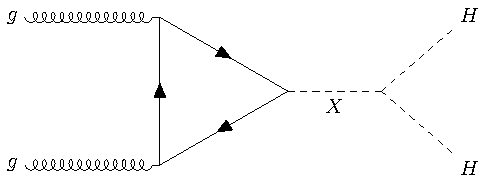
\includegraphics[width=0.48\textwidth]{figures/feyn-scalar.pdf}
		 }
\subfloat[]{\label{fig:grav-diagram}
		  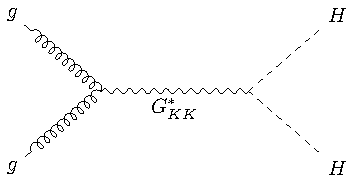
\includegraphics[width=0.48\textwidth]{figures/feyn-graviton.pdf}
		 }

\caption{\label{fig:ggF-diagrams-res} Representative diagrams for the gluon-gluon fusion production of spin-0 ($X$) 
and spin-2 ($G_{KK}^{*}$) resonances which decay to two Standard Model Higgs bosons.The spin-0 resonance considered
for this thesis is a generic narrow width resonance which may be interpreted in the context of 
two Higgs doublet models~\cite{2HDM}, whereas the spin-2 resonance is considered as a Kaluza-Klein graviton within the bulk Randall-Sundrum (RS) model~\cite{Gravitons,Carvalho}.}
\end{figure}

\begin{figure}[ht]
\centering
\subfloat[]{\label{fig:ggF-tri}
		  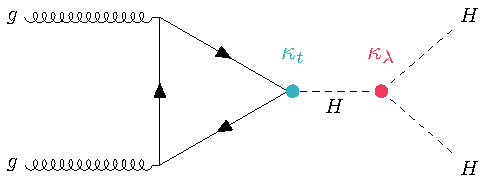
\includegraphics[width=0.48\textwidth]{figures/ggF-tri.pdf}
		 }
\subfloat[]{\label{fig:ggF-box}
		  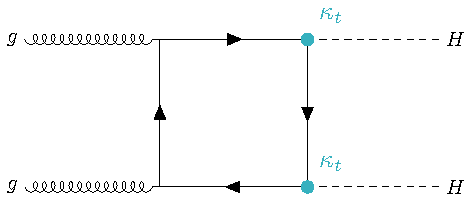
\includegraphics[width=0.48\textwidth]{figures/ggF-box.pdf}
		 }

\caption{\label{fig:ggF-diagrams-nonres} Dominant contributing diagrams for non-resonant gluon-gluon fusion production of 
$HH$. $\kappa_{\lambda}$ and $\kappa_{t}$ represent ratios of the Higgs self-coupling and coupling to top quarks 
respectively, relative to the values predicted by the Standard Model.}
\end{figure}

As shown in Chapter \ref{chap:intro-SM}, the Higgs coupling to fermions scales with particle mass. 
As the top quark has a mass of \SI{173}{\GeV}, whereas the $\higgs$ has a mass of \SI{125}{\GeV}, such that 
\HepProcess{\higgs \to \Pqt\Paqt} is kinematically disfavored, \HepProcess{\higgs \to \Pqb\Paqb} is the dominant 
fermionic Higgs decay mode, and, in fact, 
the dominant overall decay mode, with a branching fraction of around 58~\%. The dominant top quark Yukawa coupling to 
the \higgs does play a role in \higgs production, however -- gluon-gluon fusion is dominated by processes including 
a top loop.

The single \higgs properties translate to $\higgs\higgs$ production, with \HepProcess{\higgs\higgs \to \bbbb} accounting
for around 34~\% of all $\higgs\higgs$ decays. The \higgs\higgs branching fractions are shown in Figure \ref{fig:hh-br}.
\begin{figure}[ht]
\centering
\subfloat{
		  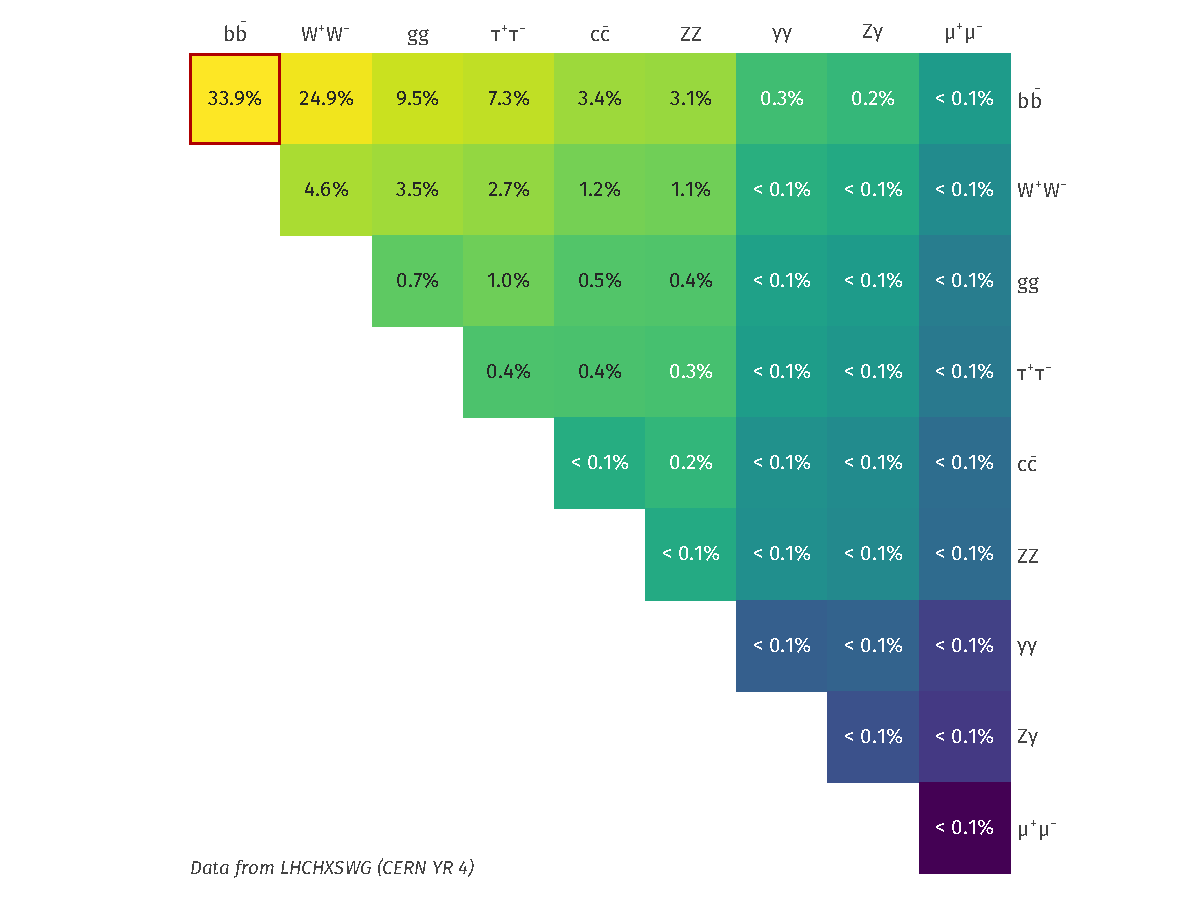
\includegraphics[width=0.8\textwidth]{figures/branching-ratios.pdf}
		 }
\caption{\label{fig:hh-br} Illustration of dominant $HH$ branching ratios. $HH\rightarrow \bbbb$ is the most common 
decay mode, representing 34~\% of all $HH$ events produced at the LHC.}
\end{figure}

\section{Resonant $HH$ Searches}
Resonant di-Higgs production is predicted in a variety of extensions to the
Standard Model. In particular, this thesis presents searches for both spin-0 and spin-2 resonances. 
The decay of spin-1 resonances to two identical spin-0 bosons is prohibited, as the final state 
must correspondingly be symmetric under particle exchange, but this process would require 
orbital angular momentum $\ell = 1$, and thus an anti-symmetric final state.
Each model considered here is implemented in a particular theoretical context, but set up experimental results 
for generic searches.

The spin-2 signal considered is implemented within the bulk Randall-Sundrum (RS)
model~\cite{Gravitons,Carvalho}, which features spin-2 Kaluza-Klein gravitons,
\PGrav, that are produced via gluon-fusion and which may decay to a pair of Higgs bosons. The model
predicts such gravitons as a consequence of warped extra dimensions, and is correspondingly 
parametrized by a value $c=k/\overline{M}_{\mathrm{Pl}} = 1$, where $k$ describes a curvature 
scale for the extra dimension and $\overline{M}_{\mathrm{Pl}}$ is the Planck mass. The model considered 
here has $c=1.0$. However, this model was considered in the early Run 2 $HH$ analyses~\cite{HDBS-2018-58},
and was excluded across much of the relevant mass range. 

The primary theoretical focus of this work is therefore the spin-0 result, which 
is implemented as a generic resonance with width below detector resolution. Scalar 
resonances are interesting, for instance, in the context of two Higgs doublet models~\cite{2HDM}, which 
posit the existence of a second Higgs doublet. This leads to the existence of five scalar
particles in the Higgs sector -- roughly, two complex doublets provide eight degrees of freedom, three of 
which are ``eaten'' by the electroweak bosons, leaving five degrees of freedom which may correspond
to physical fields.

\section{Non-resonant $HH$ Searches}
Non-resonant $HH$ production is predicted by the Standard Model via the trilinear coupling discussed above,
as well as via production in a fermion loop. More explicitly, after electroweak symmetry breaking, we have
\begin{align}
\mathcal{L}_{SM} &\supset -\lambda v^2h^2 - \lambda v h^3 - \frac{1}{4}\lambda h^4\\
&= -\frac{1}{2}m_{H}^2 - \lambda_{HHH}^{SM}vh^3 - \lambda_{HHHH}^{SM}h^4
\end{align}
where $m_{H} = \sqrt{2\lambda v^2}$ so that 
\begin{equation}
\lambda_{HHH}^{SM} = \frac{m_{H}^2}{2v^2}.
\end{equation}
The mass of the SM Higgs boson has been experimentally measured to be \SI{125}{\GeV}~\cite{Higgs-Mass}, and 
the vacuum expectation value $v=$\SI{246}{\GeV} has a precise determination from the muon lifetime~\cite{Higgs-vac}. 
This coupling is therefore precisely predicted in the Standard Model, such that an observed deviation from 
this prediction would be a clear sign of new physics. 

The relevant diagrams for non-resonant $HH$ production are shown in Figure \ref{fig:ggF-diagrams-nonres}.
Notably, the diagrams \emph{interfere} with each other, which can be easily seen by counting the fermion lines. 
A detailed theoretical discussion is provided by, e.g.~\cite{Dawson-2015}.

For the searches presented here, the quark couplings to the Higgs are considered to be consistent with the Standard 
Model value, with measurements of the dominant top Yukawa coupling left to more sensitive direct measurements, e.g. from 
$t\bar{t}$ final states~\cite{top-Yukawa}. Variations of the trilinear coupling away from the Standard 
Model are considered, however. Such variations are parametrized via 

\begin{equation}
\kappa_{\lambda} = \frac{\lambda_{HHH}}{\lambda_{HHH}^{SM}}
\end{equation}
where $\lambda_{HHH}$ is a varied coupling and $\lambda_{HHH}^{SM}$ is the Standard Model prediction.
As this variation comes as a prefactor only with the \emph{triangle} diagram, significant and interesting 
effects are observed due to the interference. Examples of the impact of this tradeoff on the di-Higgs invariant 
mass are shown in Figure \ref{fig:kl-shapes}. Generally speaking, the triangle diagram contributes more at low mass, 
while the box diagram contributes more at high mass. 

\begin{figure}[ht]
\centering
\subfloat{
		  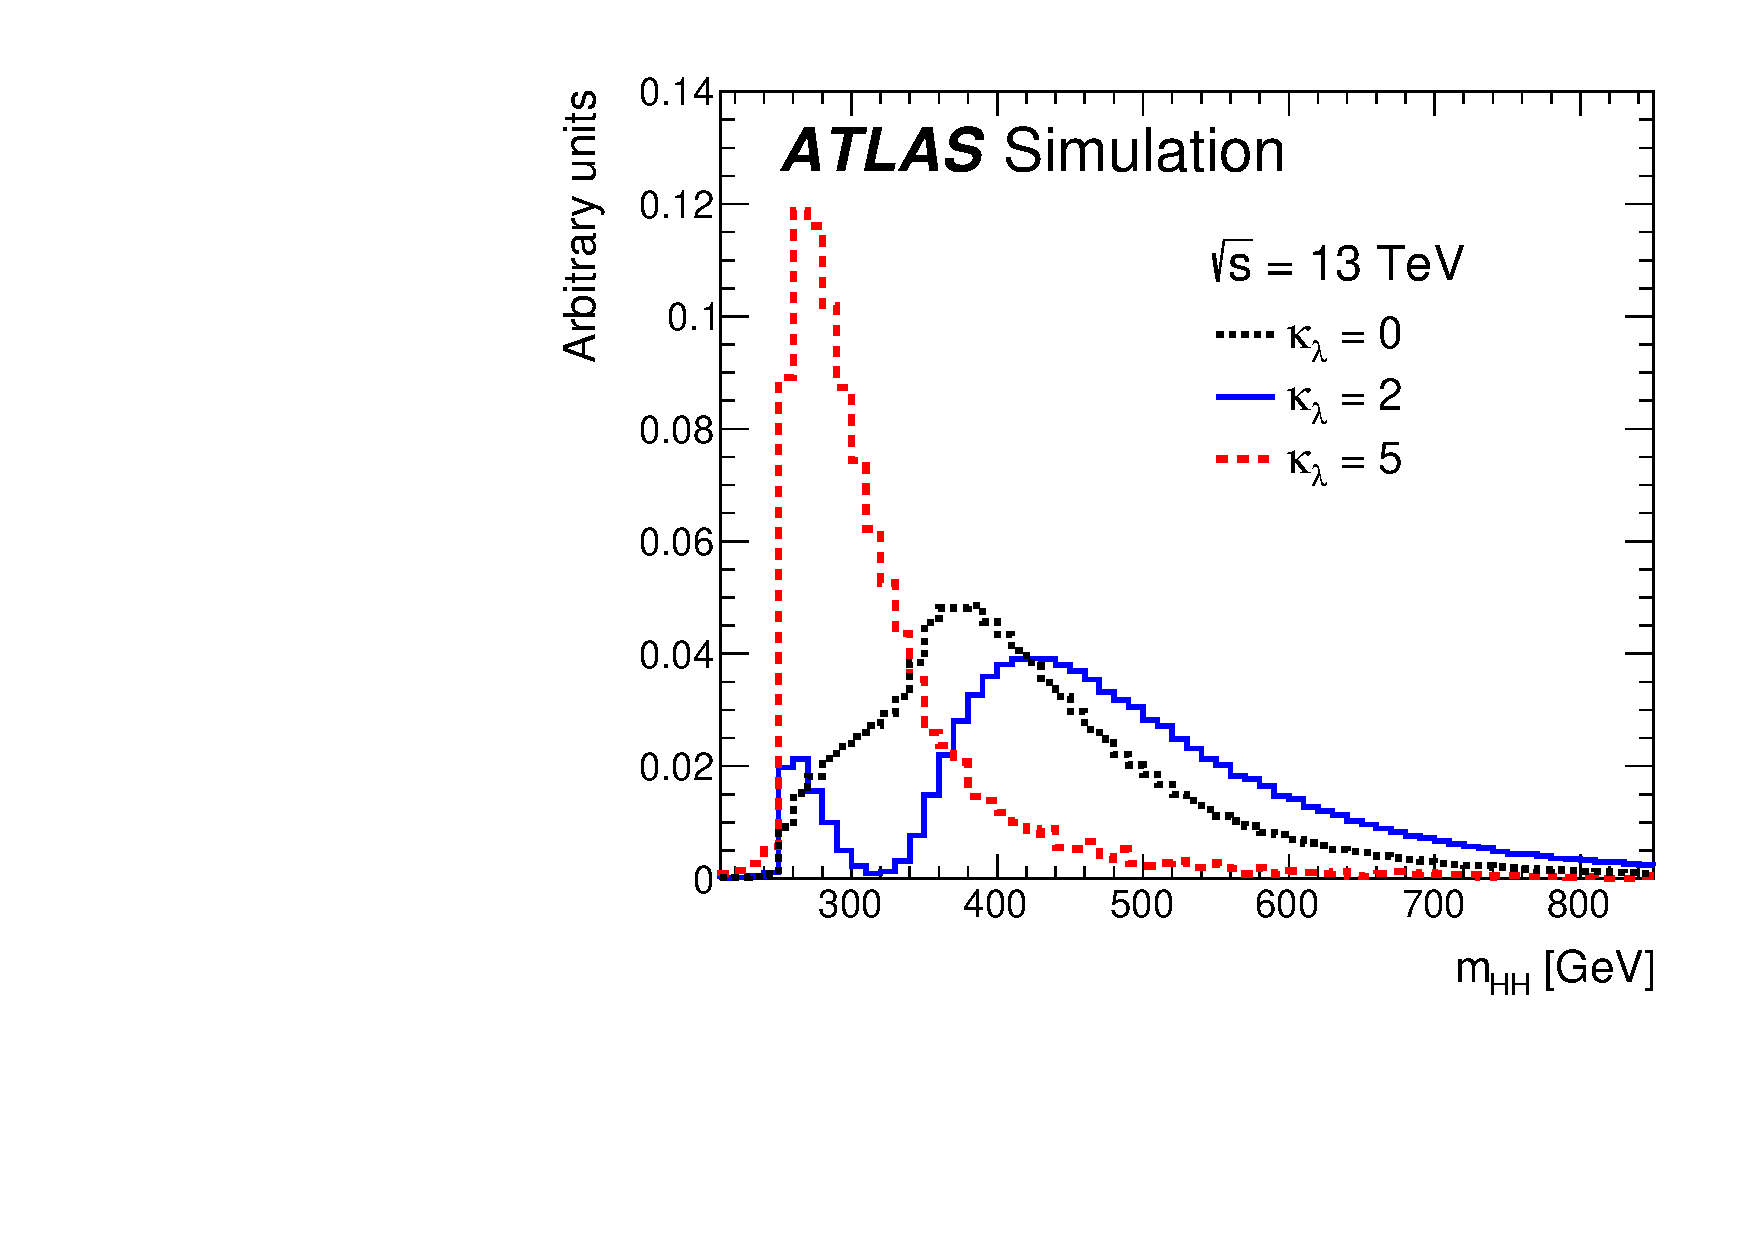
\includegraphics[width=0.48\textwidth]{figures/kl-0-2-5-combination.pdf}
		 }
\subfloat{
		  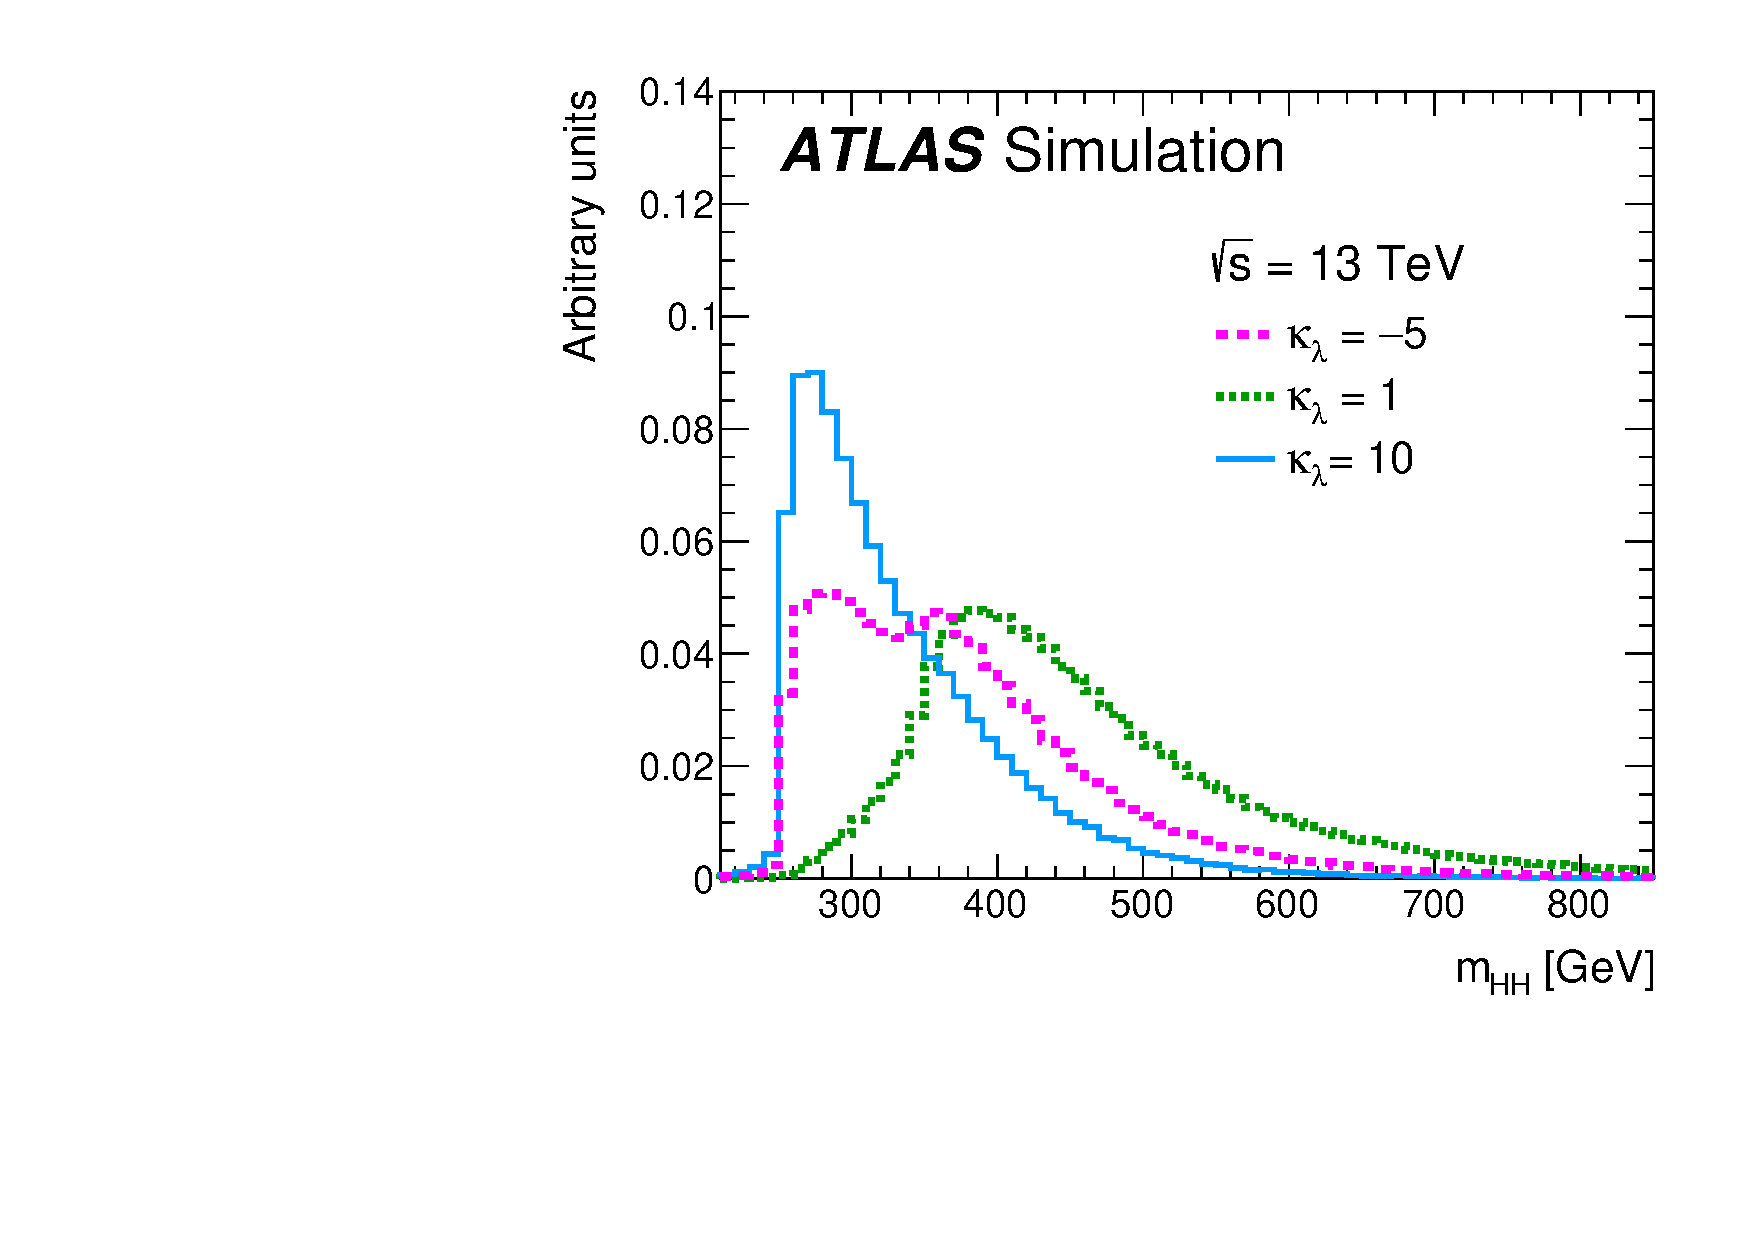
\includegraphics[width=0.48\textwidth]{figures/kl--5-1-10-combination.pdf}
		 }
\caption{\label{fig:kl-shapes} Monte Carlo generator level $m_{HH}$ distributions for various values of 
$\kappa_{\lambda}$, demonstrating the impact of the interference between the two diagrams of Figure \ref{fig:ggF-diagrams-nonres} 
on the resulting $m_{HH}$ distribution. For $\kappa_{\lambda} = 0$ there is no triangle diagram contribution, 
demonstrating the shape of the box diagram contribution, whereas for $\kappa_{\lambda}=10$, the triangle diagram 
dominates, with a strong low mass peak. The interplay between the two is quite evident for other values, resulting in, 
e.g., the double peaked structure present for $\kappa_{\lambda} = 2$ (near maximal destructive interference) and $\kappa_{\lambda}=-5$. At $\kappa_{\lambda}=5$, the interference leads to a deficit at high $m_{HH}$, resulting in a narrower distribution (and thus a more pronounced low mass peak) than the $\kappa_{\lambda}=10$ case. ~\cite{HDBS-2018-58}}
\end{figure}

From a quick analysis of Figure \ref{fig:ggF-diagrams-nonres}, one may see that, at leading order, the box diagram, $B$ 
has amplitude proportional to $\kappa_{t}^2$, defined as the ratio of the top Yukawa coupling to the value 
predicted by the Standard Model, whereas the triangle diagram, $T$ has amplitude proportional to 
$\kappa_{t}\kappa_{\lambda}$. Therefore, the cross section is proportional to 
\begin{align}
\sigma(\kappa_{t}, \kappa_{\lambda}) &= |A(\kappa_{t}, \kappa_{\lambda})|^2 \\
&\sim |\kappa_{t}^2B +\kappa_{t}\kappa_{\lambda}T|^2\\
&= \kappa_{t}^4|B|^2 + \kappa_{t}^3\kappa_{\lambda}(BT+TB) + \kappa_{t}^2\kappa_{\lambda}^2|T|^2,
\end{align} 
and thus non-resonant $HH$ production cross section may be parametrized as a second order 
polynomial in $\kappa_{\lambda}$.

For positive values of $\kappa_{\lambda}$, due to the relative minus sign between the triangle 
and box diagrams, the interference between the two diagrams is \emph{destructive}, with a maximum interference 
near $\kappa_{\lambda} = 2.3$, corresponding to the minimum cross section prediction. One may note that the 
Standard Model value of $\kappa_{\lambda} = 1$ is not far away from this minimum -- correspondingly the 
Standard Model cross section for $HH$ production is quite small, namely \SI{31.05}{\fb} at $\sqrt{s} = \SI{13}{\TeV}$ 
for production via gluon-gluon fusion ~\cite{HH1,HH2,HH3,HH4,HH5,HH6,HH7,HH8} compared to, e.g. single Higgs 
production, with a gluon-gluon fusion production cross section of \SI{46.86}{\pb} at 
$\sqrt{s} = \SI{13}{\TeV}$~\cite{Higgsxs} roughly 1500 times larger! For negative values of $\kappa_{\lambda}$, 
the interference is constructive.

ATLAS projections~\cite{ATL-PHYS-PUB-2018-053} of $\bbbb$, $b\bar{b}\gamma\gamma$, and $b\bar{b}\tau^{+}\tau^{-}$ 
predict an expected signal strength for Standard Model $HH$ of $3.5\sigma$ with no systematic uncertainties 
and $3.0\sigma$ with systematic uncertainties using the \SI{3000}{\ifb} of data from the HL-LHC 
(around $20\times$ the full Run 2 dataset considered in this thesis), constituting an \emph{observation} of $HH$. 
As the cross section for Standard Model $HHH$ production, corresponding 
to the quartic Higgs interaction, is much smaller (around \SI{0.1}{\fb} at $\sqrt{s} = \SI{14}{\TeV}$~\cite{TripleHiggs}),
observation of triple Higgs production is even farther in the future, and so is not considered here. However this 
may be interesting for future work in a variety of Beyond the Standard Model scenarios (e.g.~\cite{HHH1,HHH2,HHH3}).

